\documentclass{beamer}

\usepackage{graphicx}
\usepackage[utf8]{inputenc}
\usepackage[T1]{fontenc}
\usepackage{lmodern}
\usepackage[english]{babel}
\usepackage{amsmath}
\usepackage{amsthm}
\usepackage{mathtools}
\usepackage{amssymb}
\usepackage{listings}
\usepackage{xparse}
\usepackage{stmaryrd}
\usepackage{geometry}
\usepackage{enumerate}
\usepackage{hyperref}
\usepackage{tikz}
\usepackage{pgfplots}
\usepackage{stmaryrd}
\usepackage[style=english]{csquotes}

\hypersetup{
    colorlinks,
    linkcolor={red!50!black},
    citecolor={blue!50!black},
    urlcolor={blue!80!black}
}

\usetikzlibrary{babel, positioning, shapes.geometric, arrows, arrows.meta}

\title{Weber-informiert: Auslandsförderung}
\author{Simon Pohmann}

\newcommand{\Z}{\mathbb{Z}}
\newcommand{\F}{\mathbb{F}}
\newcommand{\C}{\mathbb{C}}
\newcommand{\I}{\mathbb{I}}
\newcommand{\V}{\mathbb{V}}
\newcommand{\End}{\mathrm{End}}
\newcommand{\Quot}{\mathrm{Quot}}
\newcommand{\Half}{\mathcal{H}}
\newcommand{\Lattice}{\mathcal{L}}
\newcommand{\divides}{\ \mid \ }
\newcommand{\notdivides}{\ \nmid \ }
\newcommand{\Cl}{\mathrm{Cl}}
\newcommand{\K}{\mathcal{K}}
\newcommand{\p}{\mathfrak{p}}
\newcommand{\q}{\mathfrak{q}}
\newcommand{\val}{v}
\renewcommand{\l}{\mathfrak{l}}
\renewcommand{\a}{\mathfrak{a}}
\renewcommand{\b}{\mathfrak{b}}
\renewcommand{\O}{\mathcal{O}}

\newcommand\restr[2]{{
    \left.\kern-\nulldelimiterspace
    #1
    \vphantom{\big|}
    \right|_{#2}
}}

\newtheorem{remark}{Remark}

\begin{document}

\begin{frame}
    \maketitle
\end{frame}

\begin{frame}
    \frametitle{Mathematical Institute, Oxford}
    \begin{tikzpicture}[remember picture, overlay]
        \node[at=(current page.center)] {
            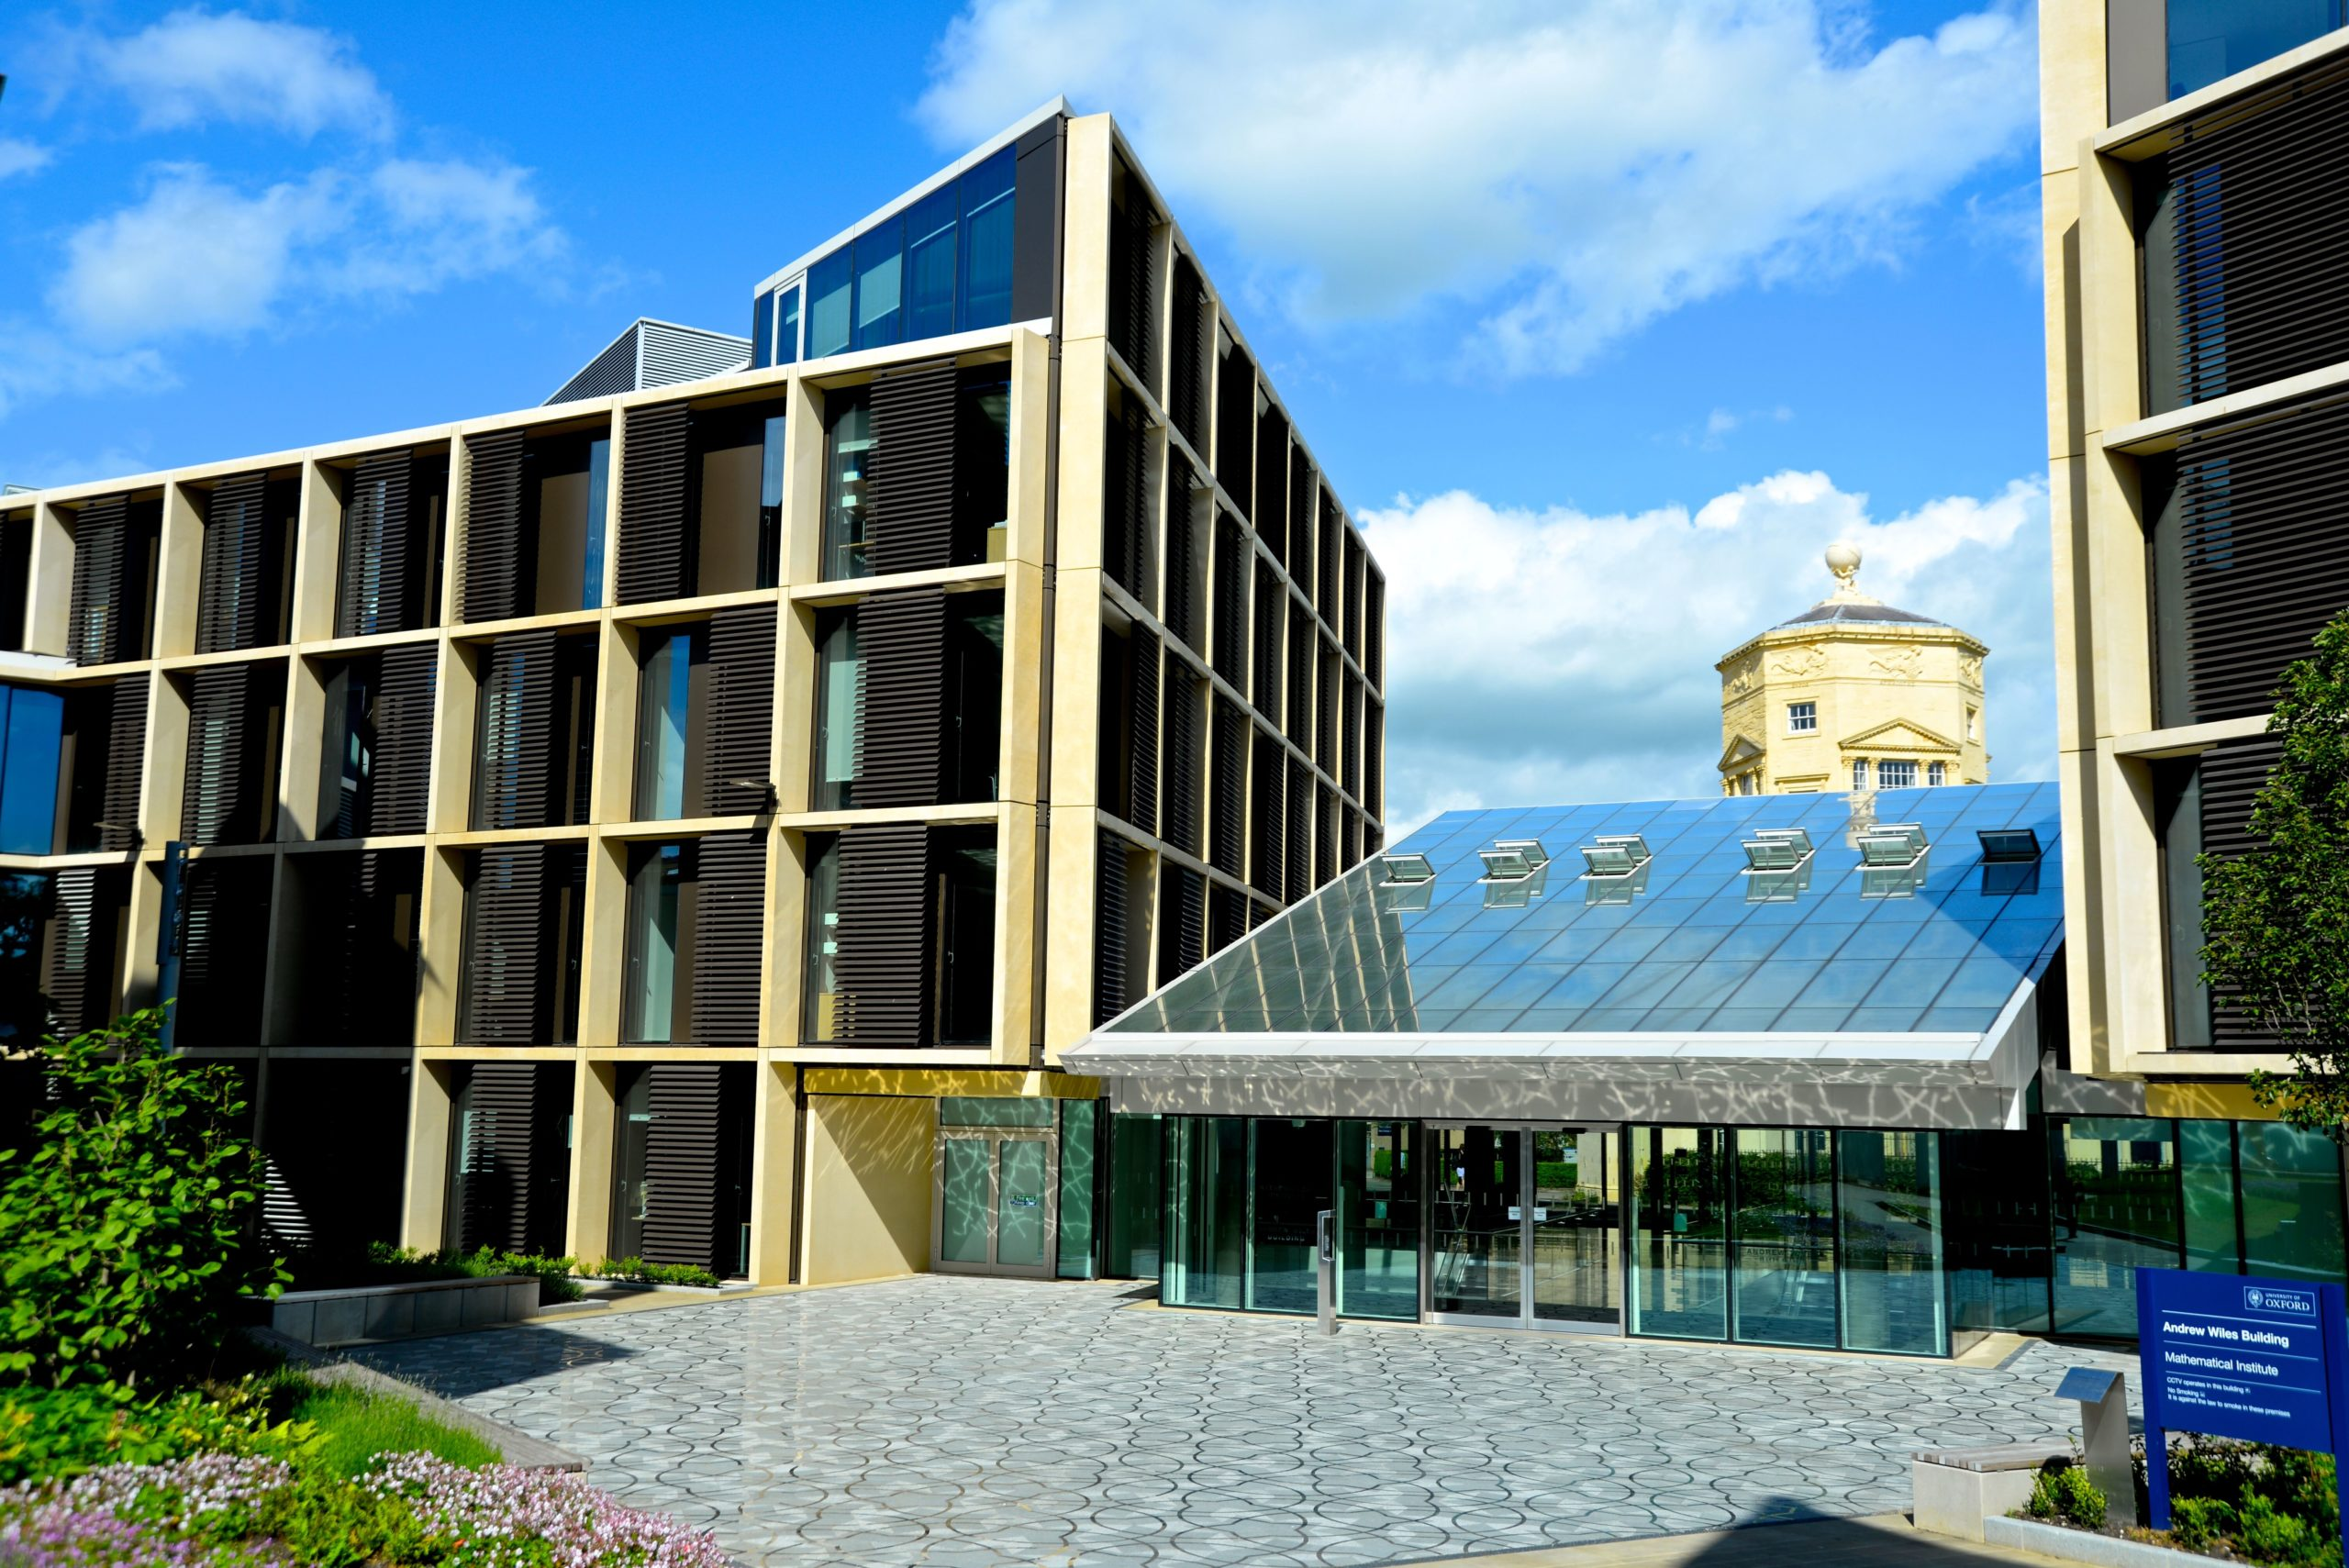
\includegraphics[keepaspectratio,height=\paperheight]{mathinstitute.jpg}
        };
    \end{tikzpicture}
\end{frame}

\begin{frame}
    \frametitle{St. Hugh's College}
    \begin{tikzpicture}[remember picture,overlay]
        \node[at=(current page.center)] {
            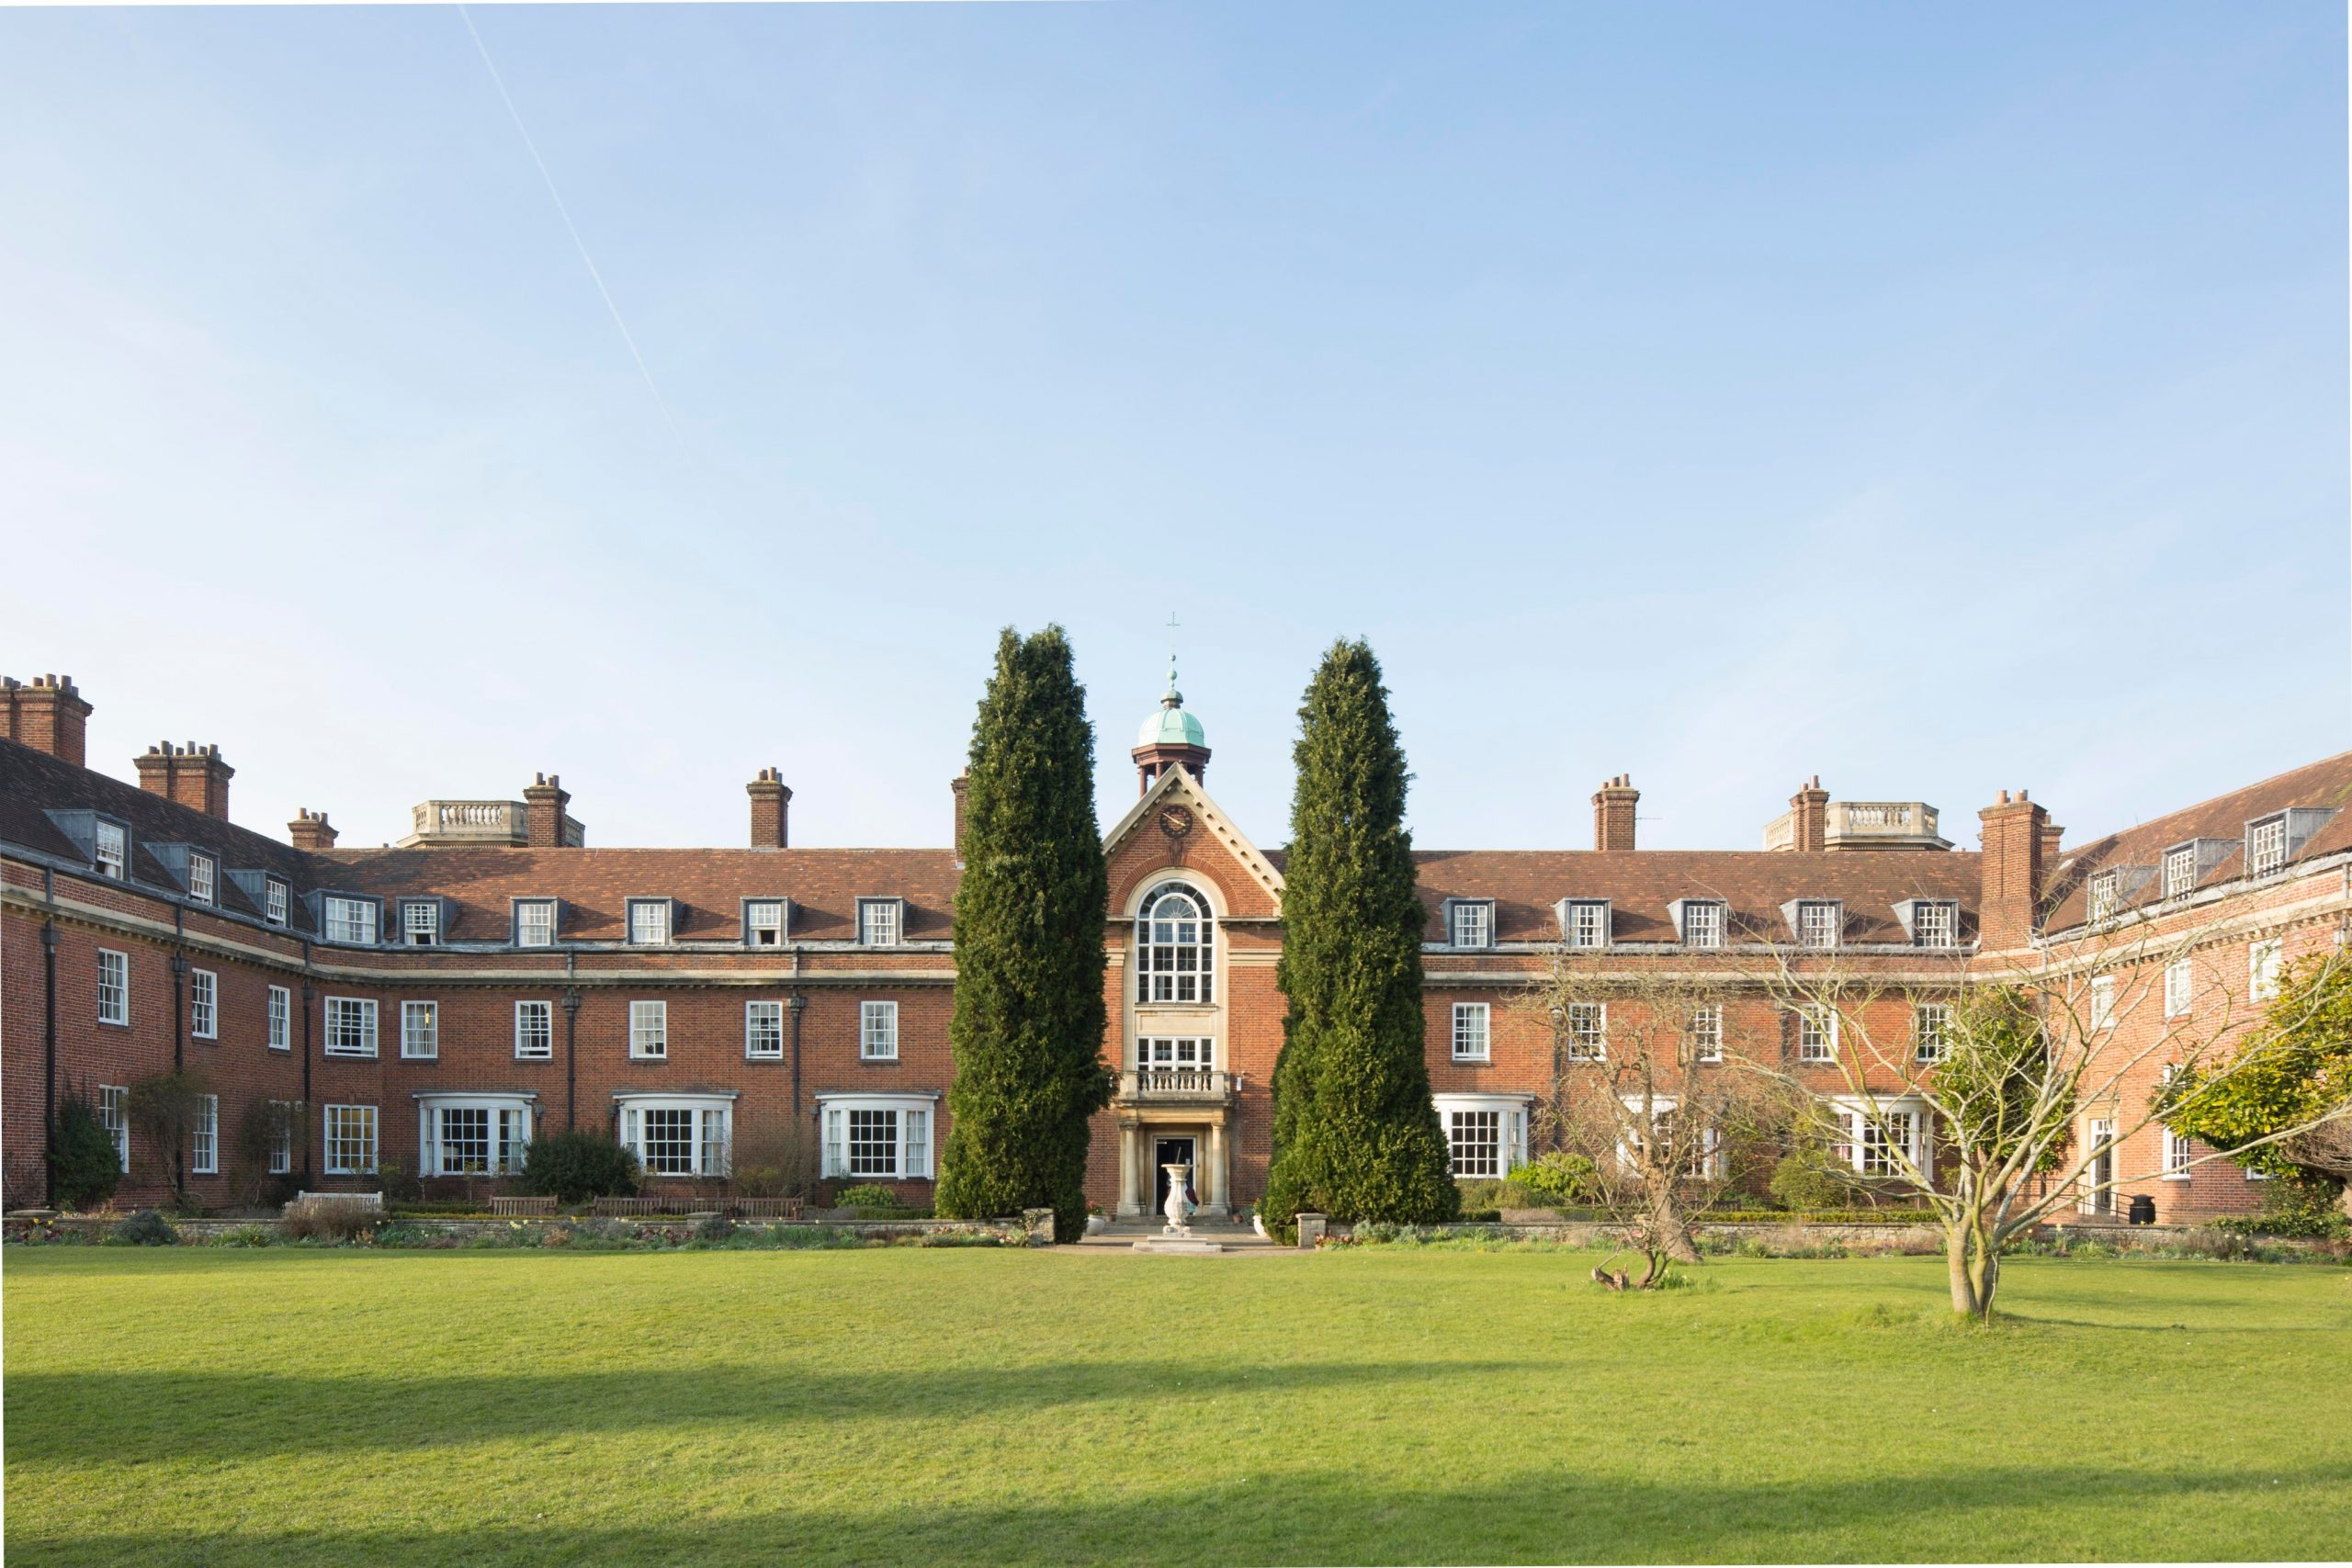
\includegraphics[keepaspectratio,height=\paperheight]{sthughs.jpg}
        };
    \end{tikzpicture}
\end{frame}

\begin{frame}
    \frametitle{Über mich}

    \begin{itemize}
        \item Bachelor in Mathe und Info in Passau
        \item Master ``Mathematics and Foundations of Computer Science'', Oxford
        \item Jetzt: PhD in Information Security, Royal Holloway (London)
    \end{itemize}
\end{frame}

\begin{frame}
    \frametitle{Master in Oxford - Timeline}

    \begin{tikzpicture}[overlay]
        \node (start) at (0, 1) {};
        \node (end) at (11, 1) {};
        \draw [->] (start) -- (end);

        \node at (1, 1.5) {Herbst 2020};
        \node at (1, 0.5) {Bewerbungsstart};

        \node at (4, 1.5) {Februar 2021};
        \node at (4, 0.5) {Bewerbungsende};

        \node at (7, 1.5) {Sommer 2021};
        \node at (7, 0.5) {Bürokratie};

        \node at (10, 1.5) {Herbst 2021};
        \node at (10, 0.5) {Studiumsbeginn};
        
        \node (start2) at (0, -3) {};
        \node (end2) at (11, -3) {};
        \draw [->] (start2) -- (end2);

        \node at (1, -2.5) {bis Dez 2021};
        \node at (1, -3.5) {Michaelmas Term};

        \node at (4, -2.5) {bis März 2022};
        \node at (4, -3.5) {Hilary Term};

        \node at (7, -2.5) {bis Jun};
        \node at (7, -3.5) {Trinity Term};

        \node at (10, -2.5) {Sommer 2022};
        \node at (10, -3.5) {Masterarbeit};
    \end{tikzpicture}
\end{frame}

\begin{frame}
    \frametitle{Diverse Informationen}

    \textbf{Bewerbung}
    \begin{itemize}
        \item Referenzschreiben
        \item Englischtest (IELTS/TOEFL)
        \item Lebenslauf \& Co
        \item Interview hängt vom Studiengang ab
    \end{itemize}
    ~\\~\\
    \textbf{Studium}
    \begin{itemize}
        \item Wohnen im College
        \item Studiengebühren: 30000€ (Brexit!)
    \end{itemize}
\end{frame}

\begin{frame}
    \frametitle{Meine Eindrücke}

    \begin{minipage}{0.5\textwidth}
        \begin{itemize}
            \item Viele Deutsche!
            \item Kurze Vorlesungszeit
            \item Master in einem Jahr
            \item College-System
            \item Namhafte Forscher
            \item Englisch
            \item Atmosphäre teilweise sehr konkurrenzbetont
            \item Viele Vorlesungen
        \end{itemize}
    \end{minipage}%
    \begin{minipage}{0.5\textwidth}
        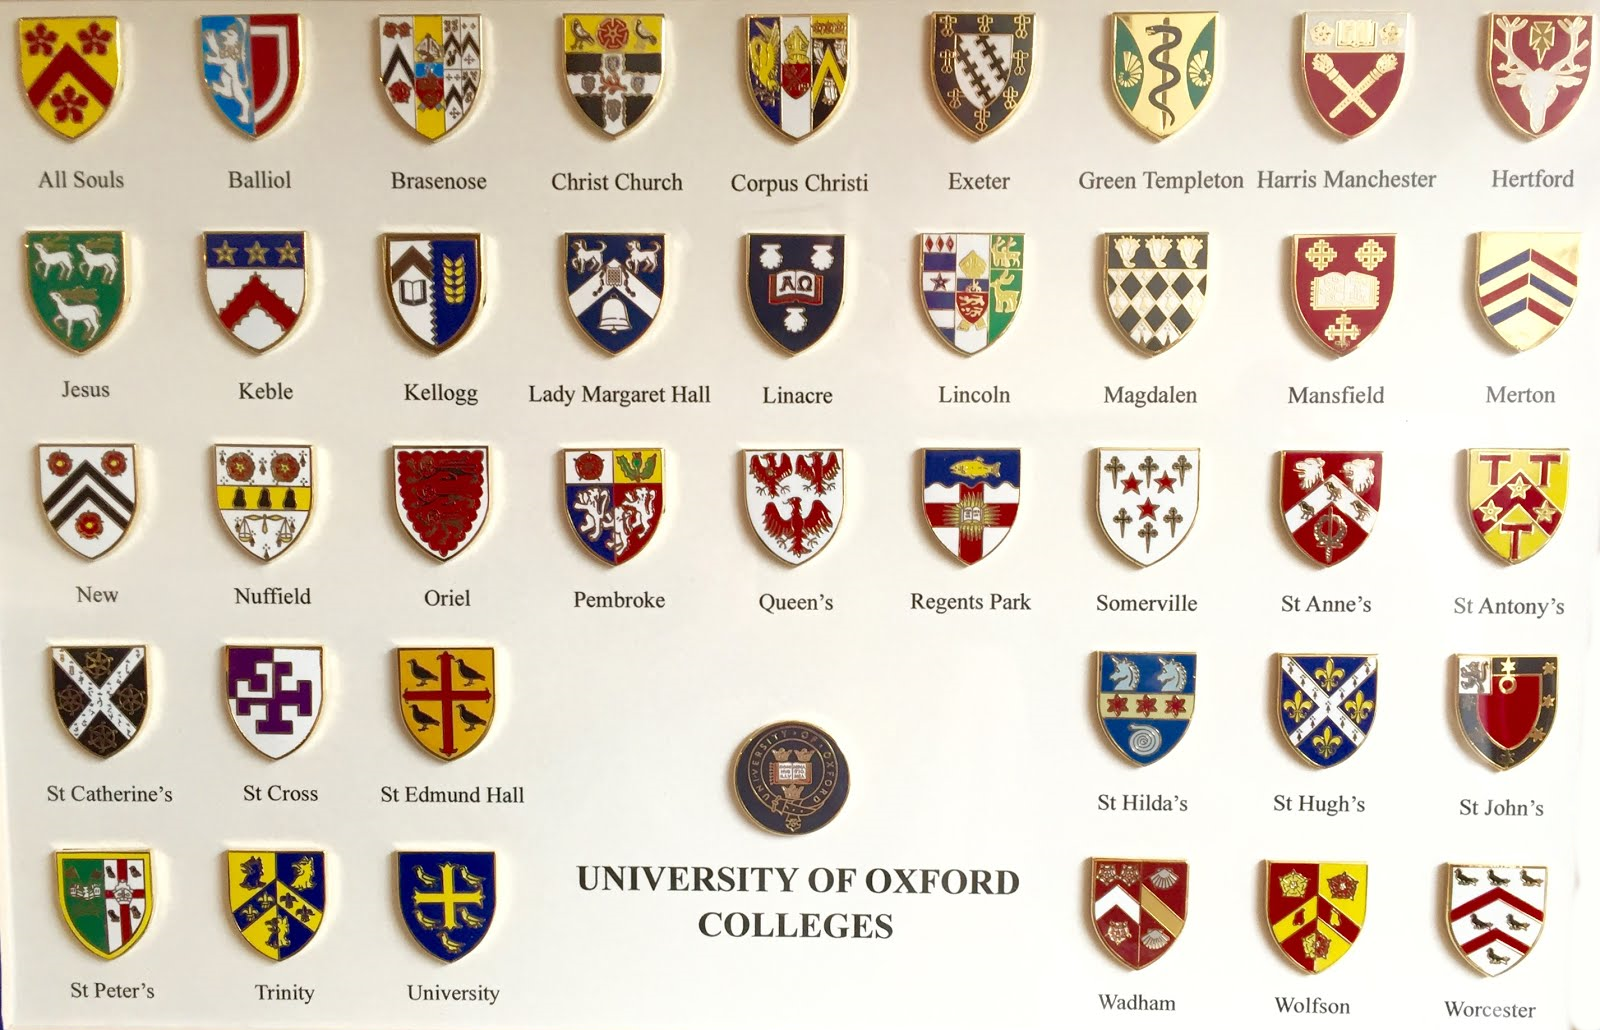
\includegraphics[width = \textwidth]{colleges.png}
        ~\\
        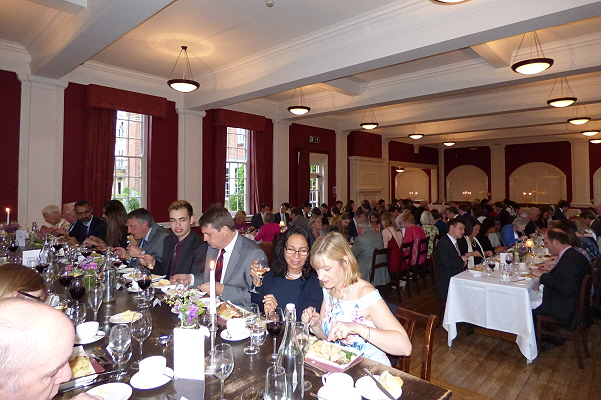
\includegraphics[width = \textwidth]{formals.png}
    \end{minipage}%
\end{frame}

\begin{frame}
    \frametitle{Royal Hollway}

    \begin{tikzpicture}[remember picture,overlay]
        \node[at=(current page.center)] {
            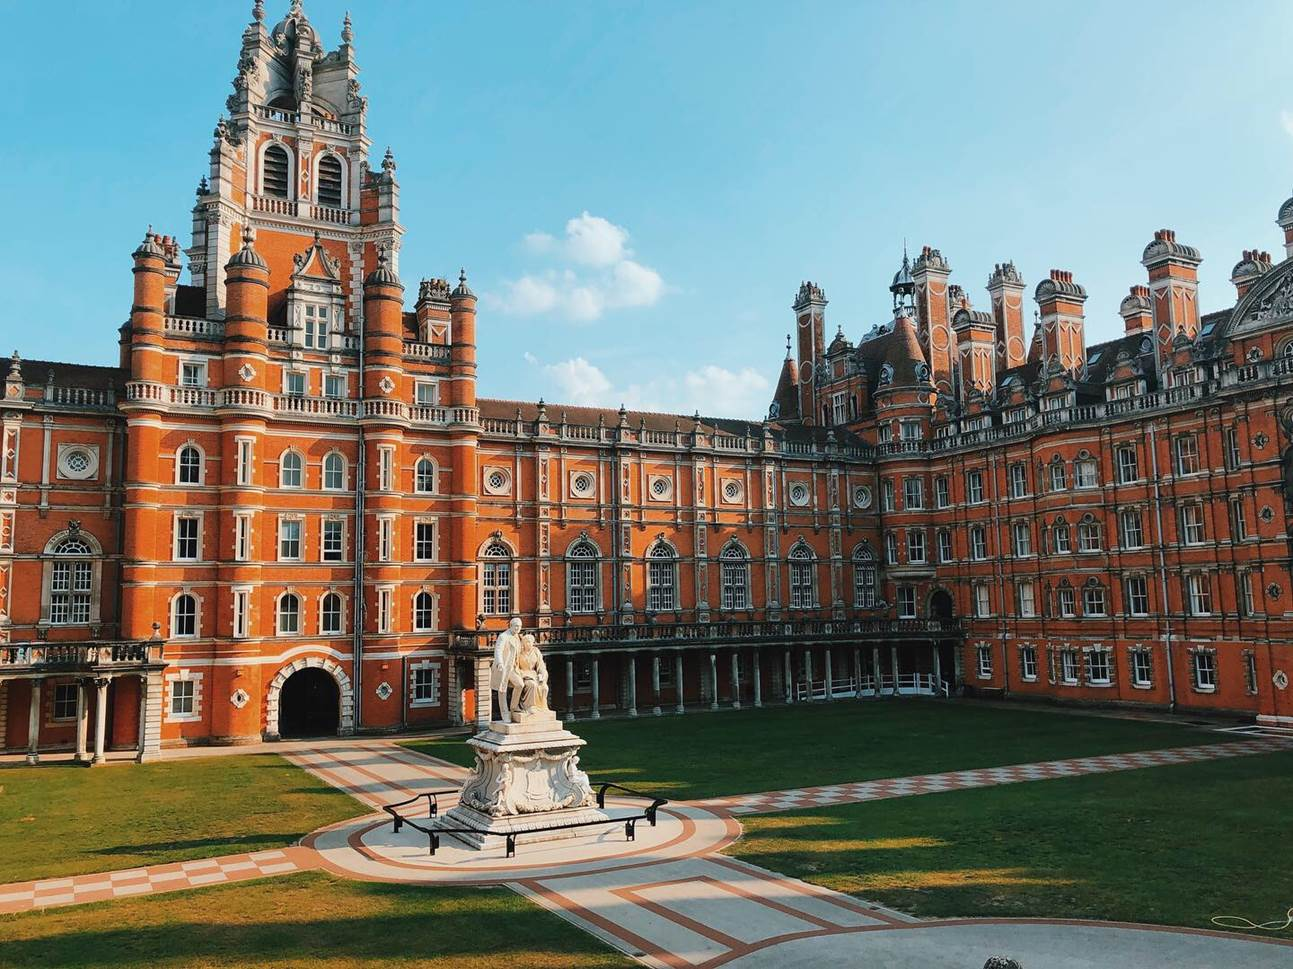
\includegraphics[keepaspectratio,height=\paperheight]{rhul.png}
        };
    \end{tikzpicture}
\end{frame}

\begin{frame}
    \begin{tikzpicture}[remember picture,overlay]
        \node[at=(current page.center)] {
            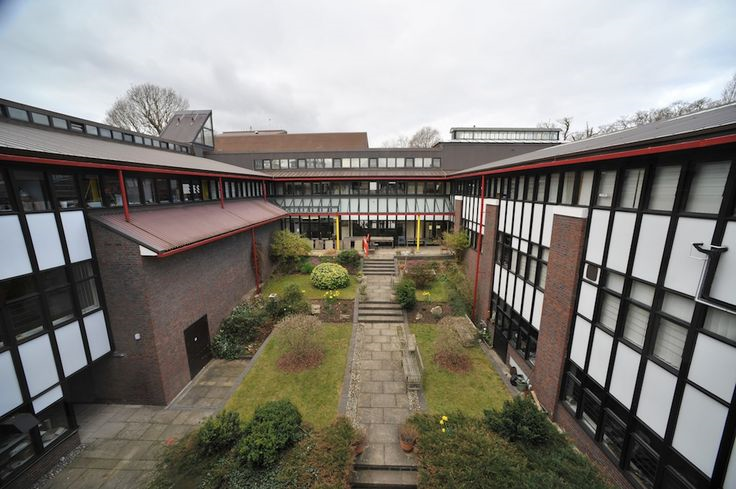
\includegraphics[keepaspectratio,height=\paperheight]{queens.png}
        };
    \end{tikzpicture}
\end{frame}

\begin{frame}
    \frametitle{Royal Holloway - Meine Eindrücke}

    \begin{minipage}{0.5\textwidth}
        \begin{itemize}
            \item Kaum gute Mathe-Vorlesungen
            \item Warme und persönliche Atmosphäre
            \item Sehr britisch
        \end{itemize}
    \end{minipage}%
    \begin{minipage}{0.5\textwidth}
        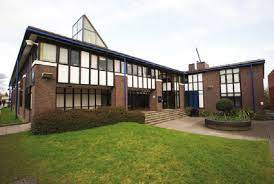
\includegraphics[width = \textwidth]{bedford.png}
        ~\\
        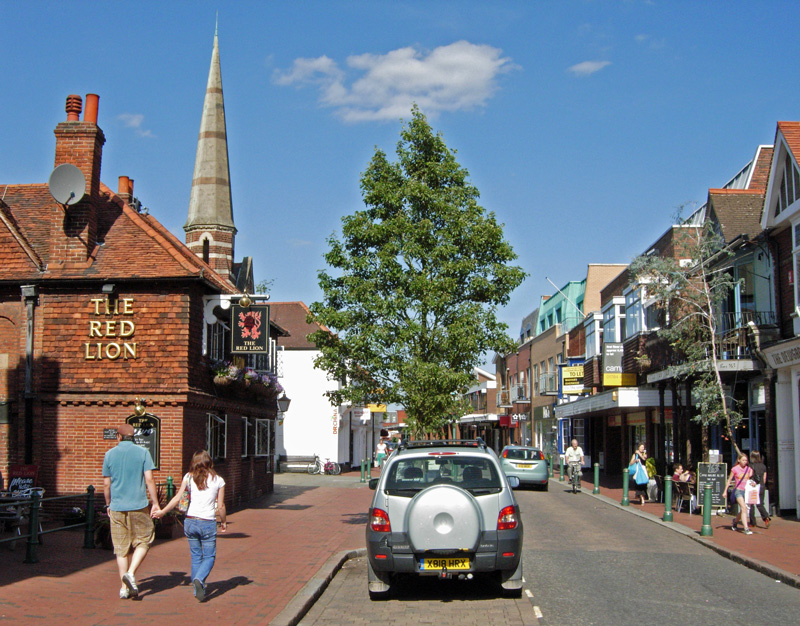
\includegraphics[width = \textwidth]{egham.png}
    \end{minipage}%
\end{frame}

\end{document}